\section{Differential Calculus}

\begin{Theorem}{
    Fundamental Lemma\footnote{\href{https://trello.com/c/byu9Pyy8}{Calculus with Analytic Geometry by George F. Simmons}, p. 680}
}{fundamental-lemma}
    Suppose that a function $z = f(x, y)$ and its partial derivatives $f_x$ and $f_y$ are defined at a point
    $(x_0, y_0)$, and also through some neighborhood of this point. Suppose further that $f_x$ and $f_y$ are continuous
    at $(x_0, y_0)$. Then the increment $\Delta z$ can be expressed in the form of

    \begin{equation}
        \Delta z = f_x(x_0, y_0)\Delta x + f_y(x_0, y_0)\Delta y + \epsilon_1\Delta x + \epsilon_2\Delta y
    \end{equation}

    where $\epsilon_1$ and $\epsilon_2 \rightarrow 0$ as $\Delta x$ and $\Delta y \rightarrow 0$
\end{Theorem}

To prove this statement, we analyze the change $\Delta z$ in 2 steps

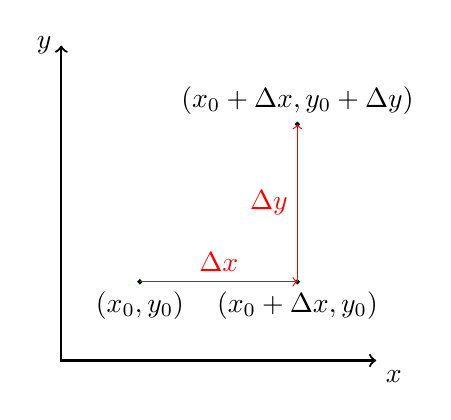
\begin{tikzpicture}
    \draw [thick, <->] (0,4) -- (0,0) -- (4,0);
    \node [below right] at (4,0) {$x$};
    \node [left] at (0,4) {$y$};

    \draw[fill] (1,1) circle [radius=0.025];
    \draw[fill] (3,1) circle [radius=0.025];
    \draw[fill] (3,3) circle [radius=0.025];

    \node [below] at (1,1) {$(x_0, y_0)$};
    \node [below] at (3,1) {$(x_0 + \Delta x, y_0)$};
    \node [above] at (3,3) {$(x_0 + \Delta x, y_0 + \Delta y)$};

    \draw [->][red] (1,1) -- node[above] {$\Delta x$} (3,1);
    \draw [->][red] (3,1) -- node[left] {$\Delta y$} (3,3);
\end{tikzpicture}

\begin{Theorem}{
    The Mean Value Theorem\footnote{\href{https://trello.com/c/byu9Pyy8}{Calculus with Analytic Geometry by George F. Simmons}, p. 76}
}{mean-value-theorem}
    Let $y = f(x)$ be a function with the following two properties:

    \begin{enumerate}
        \item $f(x)$ is continuous on the closed interval $[a, b]$; and
        \item $f(x)$ is differentiable on the open interval $(a, b)$
    \end{enumerate}

    Then there exists at least one point $c$ in the open interval $(a, b)$ such that

    \[
        f'(c) = \frac{f(b) - f(a)}{b - a}
    \]

    or equivalently,

    \[
        f(b) - f(a) = f'(c)(b - a)
    \]
\end{Theorem}

\subsection{Gradient}

\begin{equation}
    dT = \left( \frac{\partial T}{\partial x} \right) dx + \left( \frac{\partial T}{\partial y} \right) dy + \left( \frac{\partial T}{\partial z} \right) dz
\end{equation}